\documentclass[italian,a4paper]{article}
\usepackage[tight,nice]{units}
\usepackage{babel,amsmath,amssymb,amsthm,graphicx,url}
\usepackage[text={5.5in,9in},centering]{geometry}
\usepackage[utf8x]{inputenc}
\usepackage[T1]{fontenc}
\usepackage{ae,aecompl}
\usepackage[footnotesize,bf]{caption}
\usepackage[usenames]{color}
\usepackage{textcomp}
\usepackage{gensymb}
%\include{pstricks}
\frenchspacing
\pagestyle{plain}
%------------- eliminare prime e ultime linee isolate
\clubpenalty=9999%
\widowpenalty=9999
%--- definizione numerazioni
\renewcommand{\theequation}{\thesection.\arabic{equation}}
\renewcommand{\thefigure}{\arabic{figure}}
\renewcommand{\thetable}{\arabic{table}}
\addto\captionsitalian{%
  \renewcommand{\figurename}%
{Grafico}%
}
%
%------------- ridefinizione simbolo per elenchi puntati: en dash
%\renewcommand{\labelitemi}{\textbf{--}}
\renewcommand{\labelenumi}{\textbf{\arabic{enumi}.}}
\setlength{\abovecaptionskip}{\baselineskip}   % 0.5cm as an example
\setlength{\floatsep}{2\baselineskip}
\setlength{\belowcaptionskip}{\baselineskip}   % 0.5cm as an example
%--------- comandi insiemi numeri complessi, naturali, reali e altre abbreviazioni
\renewcommand{\leq}{\leqslant}
%--------- porzione dedicata ai float in una pagina:
\renewcommand{\textfraction}{0.05}
\renewcommand{\topfraction}{0.95}
\renewcommand{\bottomfraction}{0.95}
\renewcommand{\floatpagefraction}{0.35}
\setcounter{totalnumber}{5}
%---------
%
%---------
\begin{document}
\title{Problemi di analisi dati sull'effetto Faraday}
\author{\normalsize Ilaria Brivio (582116)\\%
\normalsize \url{brivio.ilaria@tiscali.it}%
\and %
\normalsize Matteo Abis (584206)\\ %
\normalsize \url{webmaster@latinblog.org}}
\date{\today}
\maketitle
%------------------
Nell'analisi dati dell'effetto Faraday si riscontrano alcune difficoltà di
cui è difficile rintracciare l'origine data la scarsa conoscenza
dell'apparato strumentale e i pochi dati disponibili. In particolare la
curva di intensità rilevata dovrebbe portare, attraverso l'interpolazione,
alla costante di Verdet. Purtroppo la determinazione della costante
dipende molto dalla regione della curva che si interpola (primo o secondo
massimo) ed è comunque molto lontana dal valore atteso di circa
$\unit[1000]{^\circ / Tm}$. La tabella seguente mostra i risultati ottenuti.
\begin{table}[h]
    \centering
    \begin{tabular}{rl}
        intervallo interpolazione ($^\circ$) & costante di Verdet
        ($\unit[]{^\circ /Tm}$)\\
        1--50 & 1202\\
        1--100 & 1196\\
        180--260 & 1120\\
        130--260 & 1131\\
    \end{tabular}
    \caption{Dati ottenuti per la costante di Verdet.}
    \label{tab:verdet}
\end{table}
Si nota che l'interpolazione non è tanto sensibile
alla porzione di curva scelta, purch\'e si rimanga intorno allo stesso
massimo.
Ulteriori informazioni si possono ricavare dai grafici dei residui relativi
a queste interpolazioni, riportiamo solo quelli relativi alle fasce 1--100 e
130--260, gli altri sono del tutto analoghi. Ogni gruppo di grafici
comprende i dati sulle quattro intensità di corrente da 0 a
\unit[3]{A}.

\begin{figure}[h]
    \begin{center}
        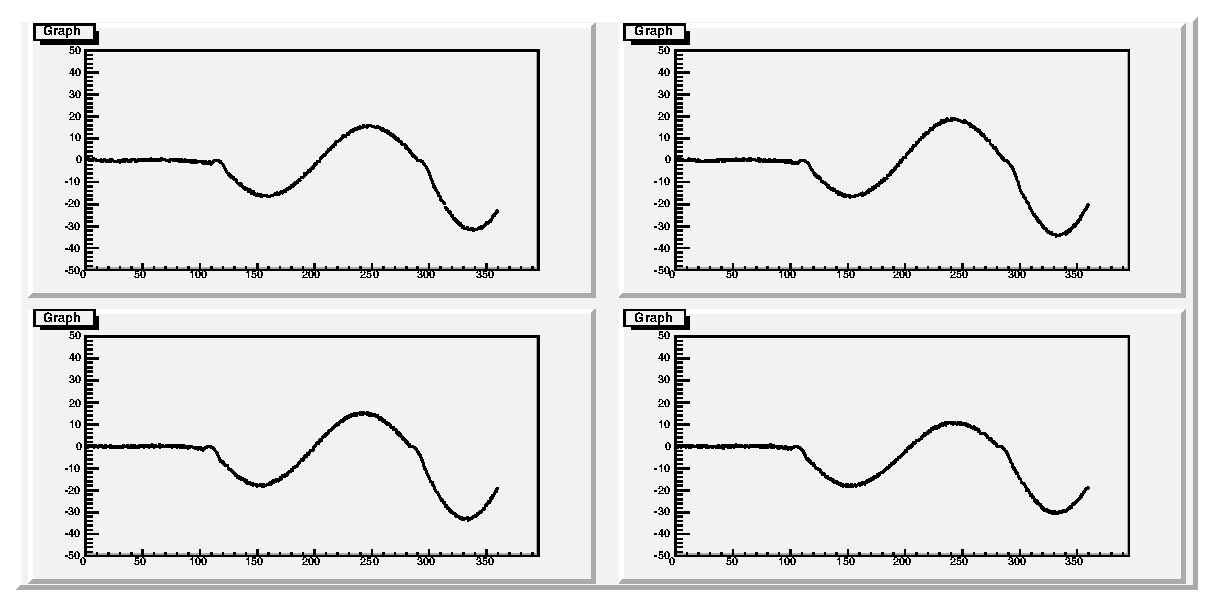
\includegraphics[height=0.4\textheight, width=.9\textwidth]{grafici/1-100r.eps}
    \end{center}
    \caption{Grafico dei residui per l'interpolazione fra 1 e
    $\unit[100]{^\circ}$}
    \label{fig:1100r}
\end{figure}
\begin{figure}[h]
    \begin{center}
        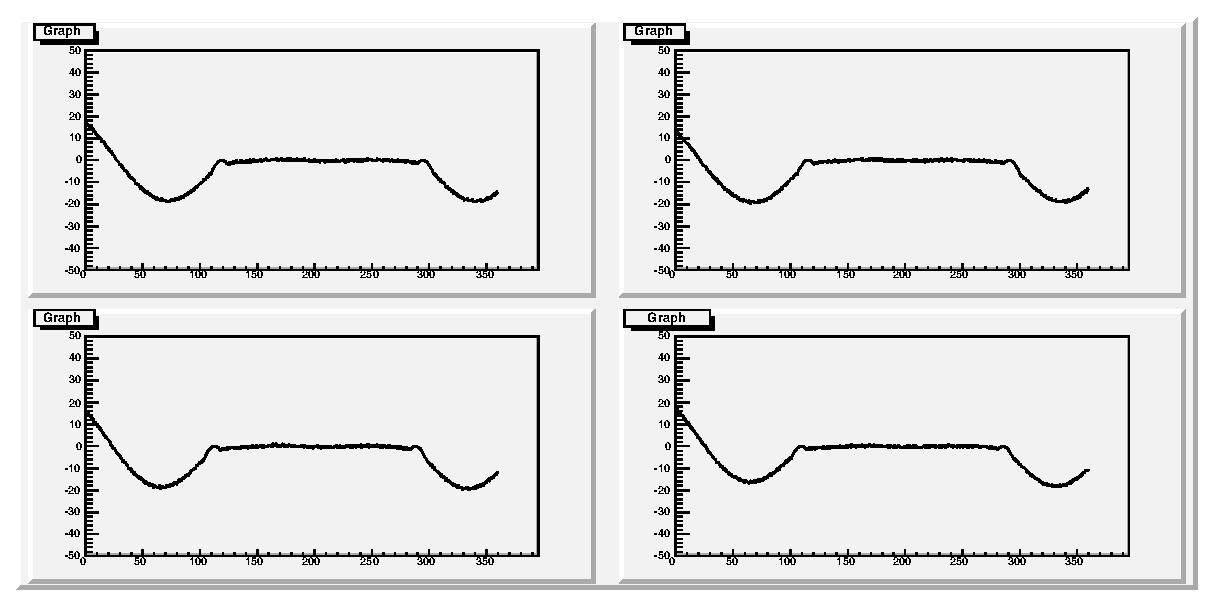
\includegraphics[height=0.4\textheight, width=.9\textwidth]{grafici/130-260r.eps}
    \end{center}
    \caption{Grafico dei residui per l'interpolazione fra 130 e
    \unit[260]{$^\circ$}}
    \label{fig:130260r}
\end{figure}

Dai grafici~\ref{fig:1100r} e~\ref{fig:130260r} \`e evidente come i parametri interpolati per la curva in un massimo siano
completamente inadeguati per quella che dovrebbe essere la stessa curva
nell'altro massimo.

Inoltre i residui presentano una certa struttura fine, anche nel tratto che
con quella scala appare piano. Li riporto nei grafici~\ref{fig:1100rbig}
e~\ref{fig:130260rbig}. Compare in tutti una sequenza a ``M'', indipendente
dall'intensità di corrente.

Tuttavia non è facile ipotizzare a cosa siano dovuti questi strani fenomeni,
non conoscendo nel dettaglio le caratteristiche di molti elementi
delicati dell'apparato strumentale, tra cui certamente possiamo
contare il fotodiodo, l'amplificatore lineare del segnale, il motore che
ruota il polaroid, l'elettronica che controlla il motore stesso e che
comunica con il computer.

In ogni caso ci sembra che da questa analisi altro non si possa
concludere se non che la costante di Verdet del campione utilizzato è tra
1100 e \unit[1200]{$^\circ$/Tm}. Si può stimare il valore come una media con
errore la semidispersione, quindi circa
\begin{equation*}
    V = \unit[1160\pm40]{^\circ/Tm}
\end{equation*}

Per completezza, riporto nei grafici finali anche quelli delle
interpolazioni sulle curve sinusoidali e dell'interpolazione lineare finale.
\begin{figure}[h]
    \begin{center}
        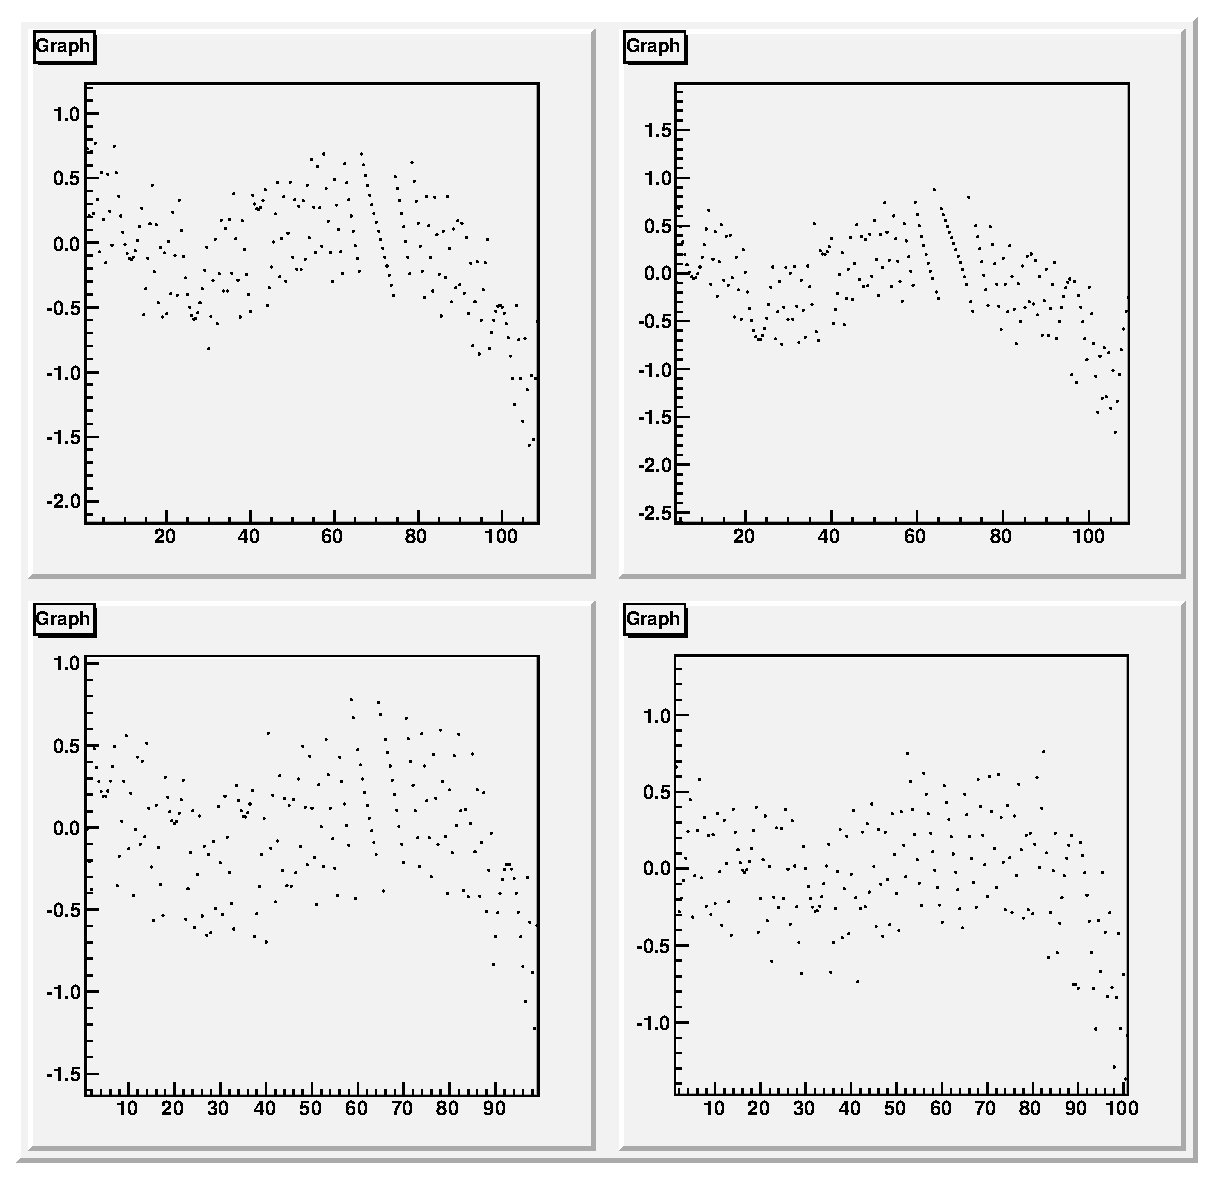
\includegraphics[height=0.4\textheight, width=.9\textwidth]{grafici/1-100r.big.eps}
    \end{center}
    \caption{Grafico dei residui 1-100$^\circ$, ingrandimento.}
    \label{fig:1100rbig}
\end{figure}

\begin{figure}[h]
    \begin{center}
        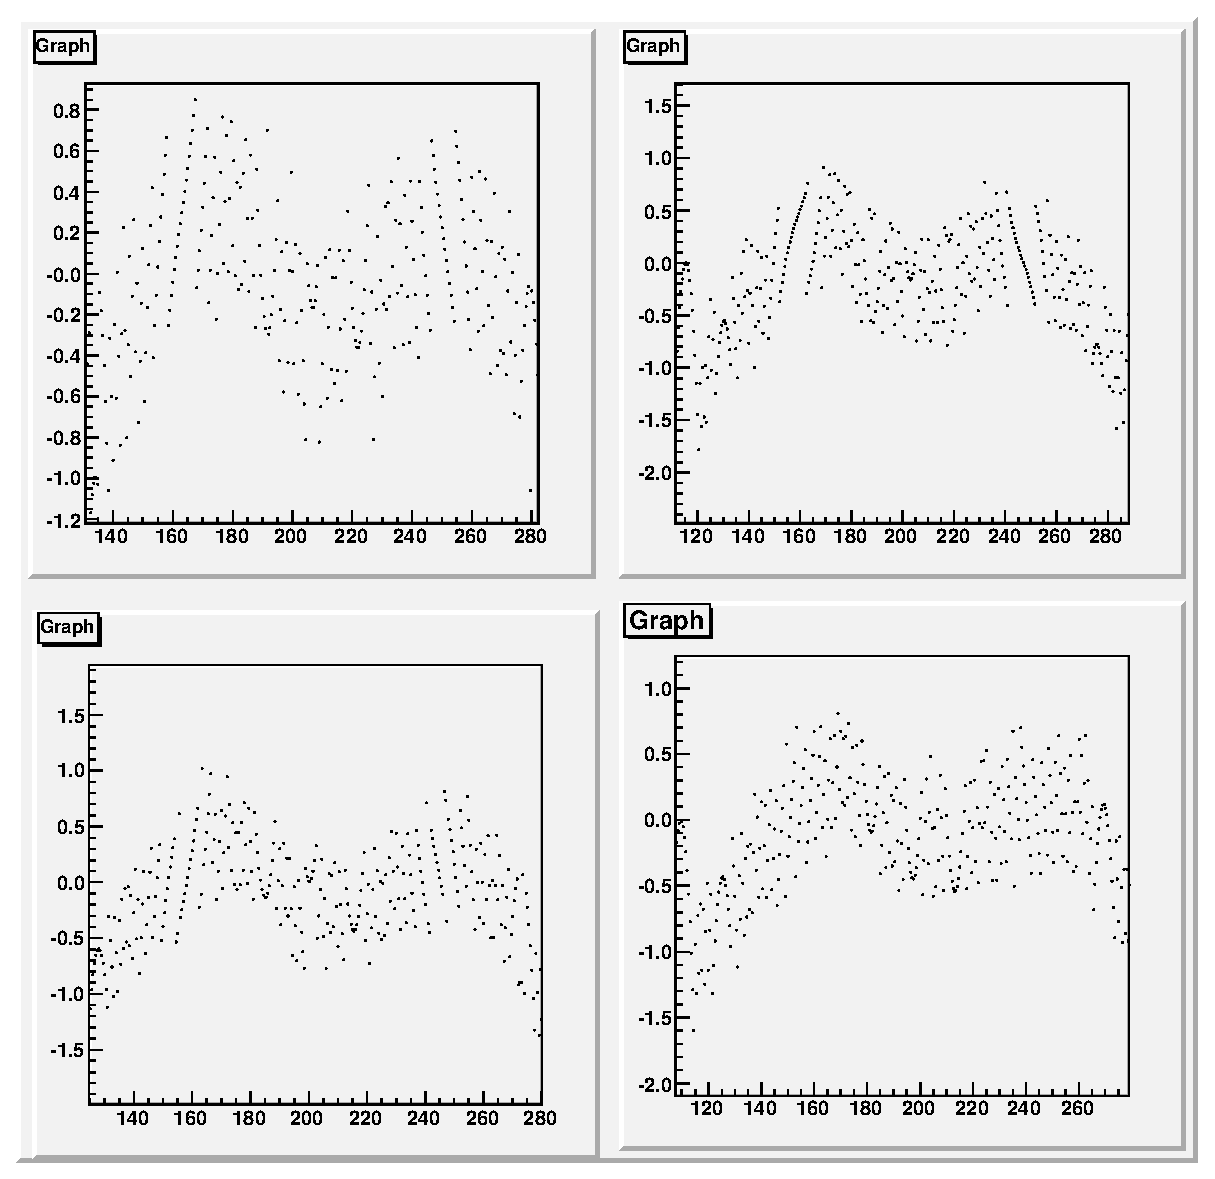
\includegraphics[height=0.4\textheight, width=.9\textwidth]{grafici/130-260r.big.eps}
    \end{center}
    \caption{Grafico dei residui 130-260$^\circ$, ingrandimento.}
    \label{fig:130260rbig}
\end{figure}

\begin{figure}[h]
    \begin{center}
        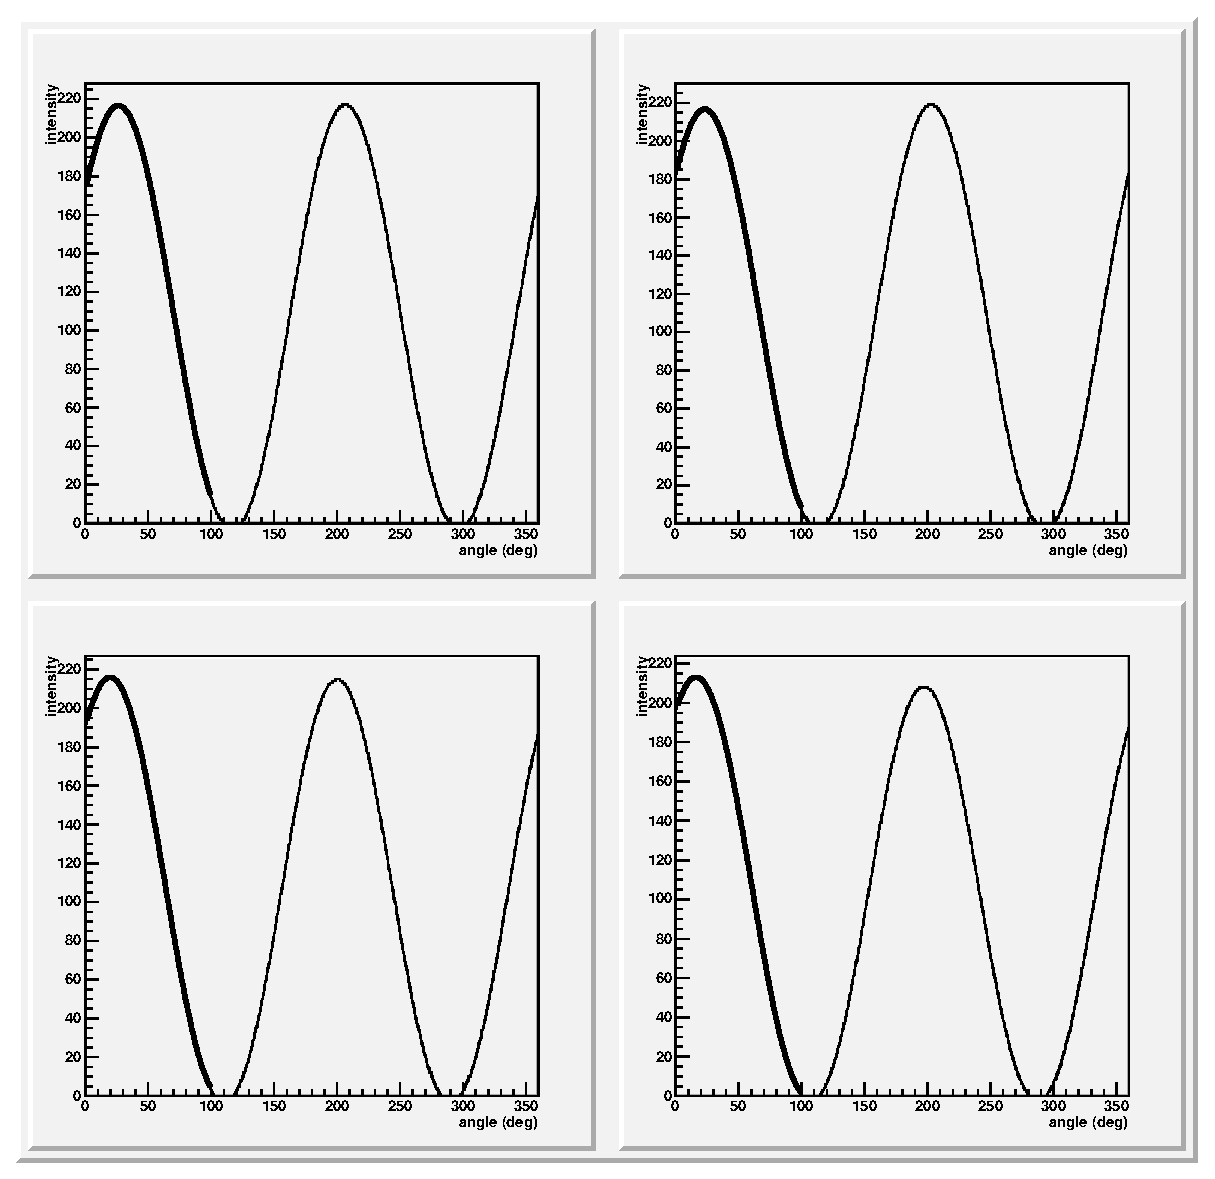
\includegraphics[height=0.4\textheight, width=.9\textwidth]{grafici/1-100g.eps}
    \end{center}
    \caption{Grafico dell'interpolazione 1-100$^\circ$.}
    \label{fig:1100g}
\end{figure}
\begin{figure}[h]
    \begin{center}
        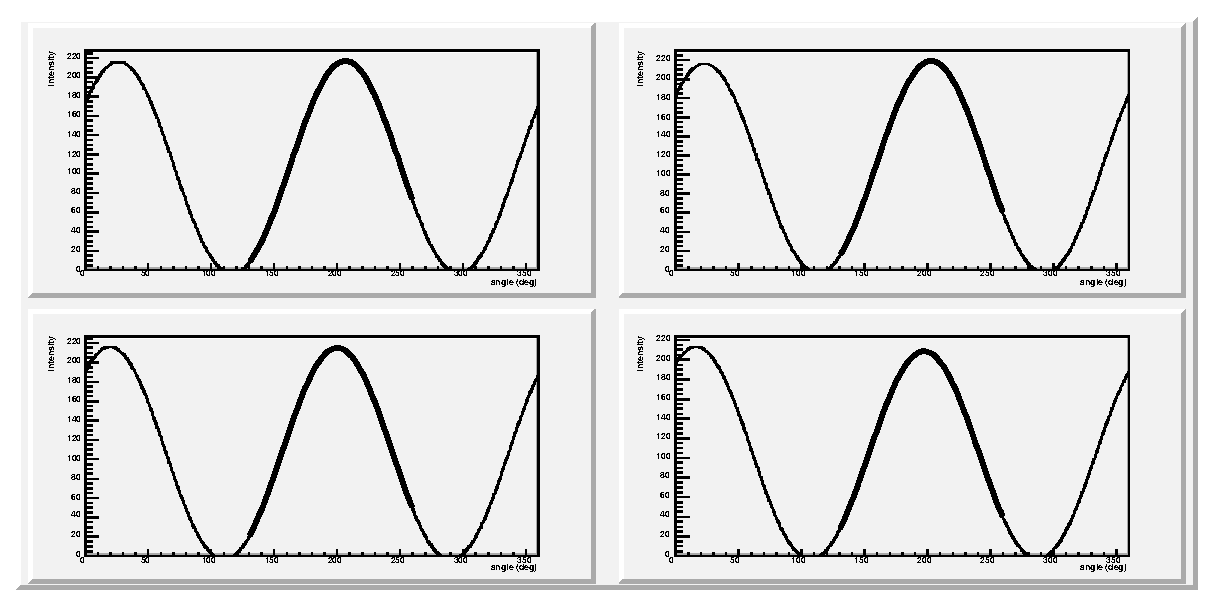
\includegraphics[height=0.4\textheight, width=.9\textwidth]{grafici/130-260g.eps}
    \end{center}
    \caption{Grafico dell'interpolazione 130-260$^\circ$.}
    \label{fig:130260g}
\end{figure}
\begin{figure}[h]
    \begin{center}
        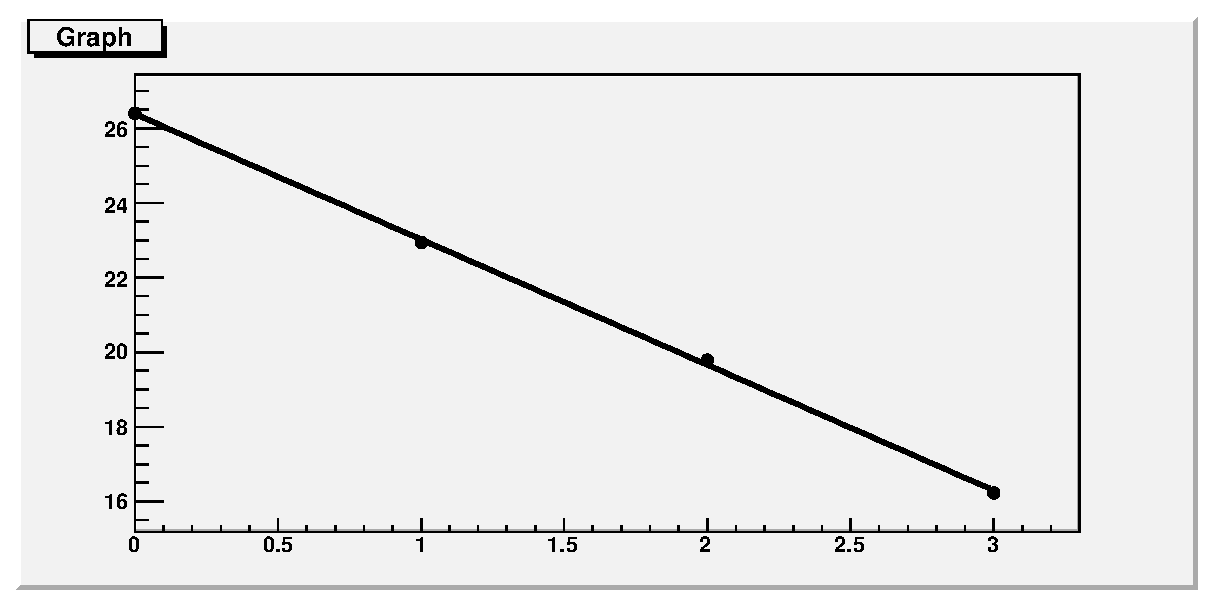
\includegraphics[height=0.4\textheight, width=.9\textwidth]{grafici/1-100verdet.eps}
    \end{center}
    \caption{Grafico dell'interpolazione lineare sui massimi alle quattro
    intensità di corrente, sempre su 1-100$^\circ$.}
    \label{fig:1100g}
\end{figure}
\begin{figure}[h]
    \begin{center}
        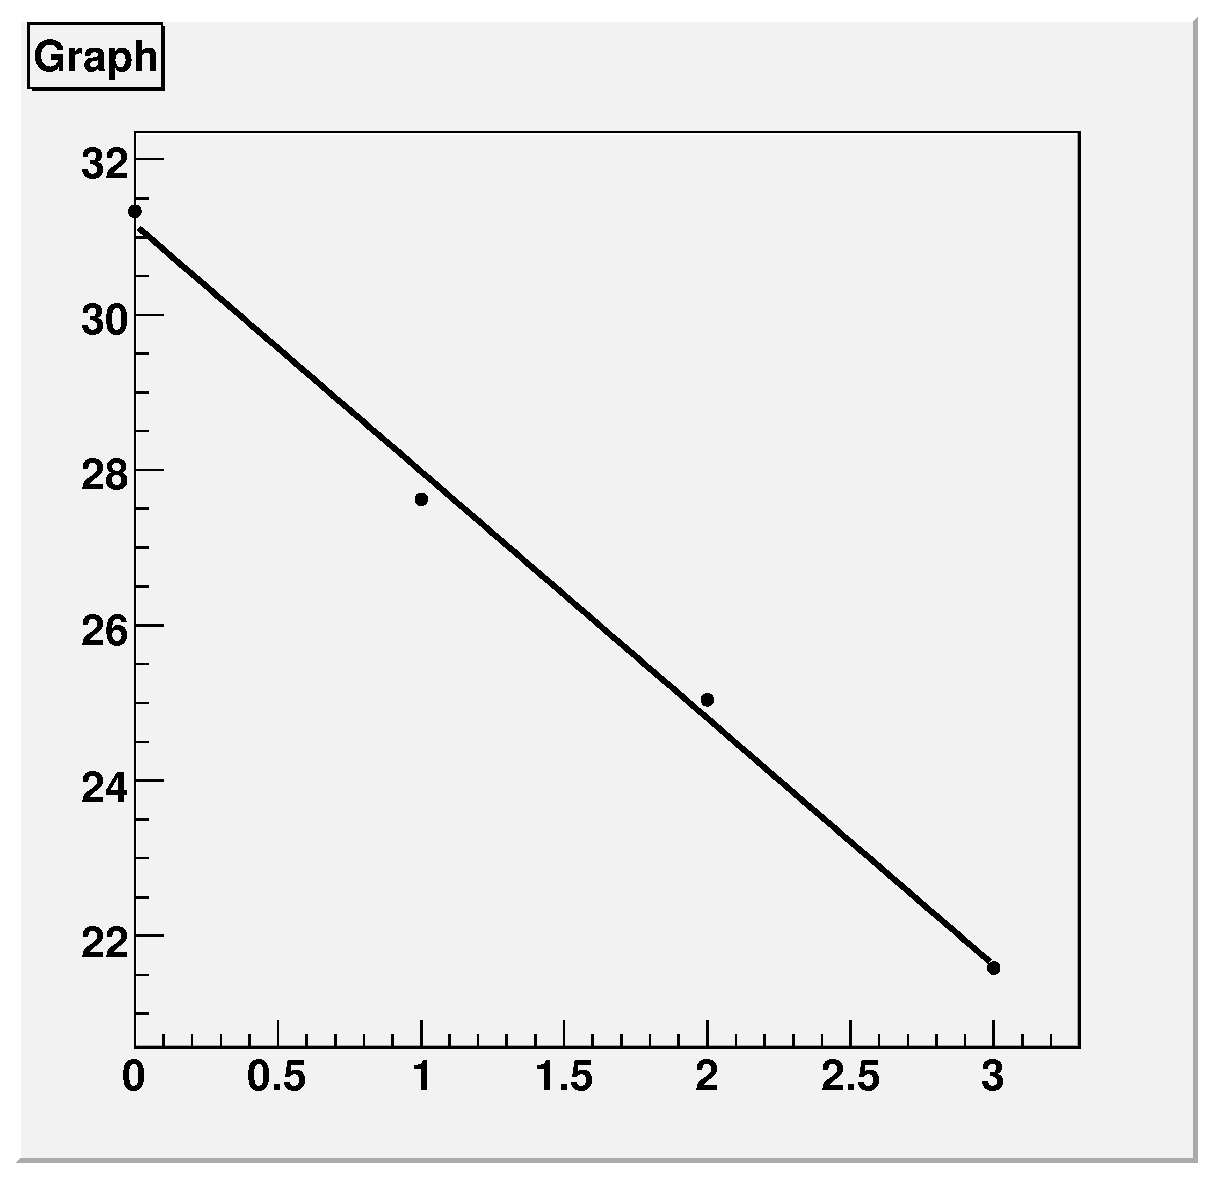
\includegraphics[height=0.4\textheight, width=.9\textwidth]{grafici/130-260verdet.eps}
    \end{center}
    \caption{Grafico dell'interpolazione lineare sui massimi alle quattro
    intensità di corrente, sempre su 130-260$^\circ$.}
    \label{fig:130260g}
\end{figure}
\end{document}
